\section*{Context and \koroibot\ project}

\begin{figure}[ht]
\centering
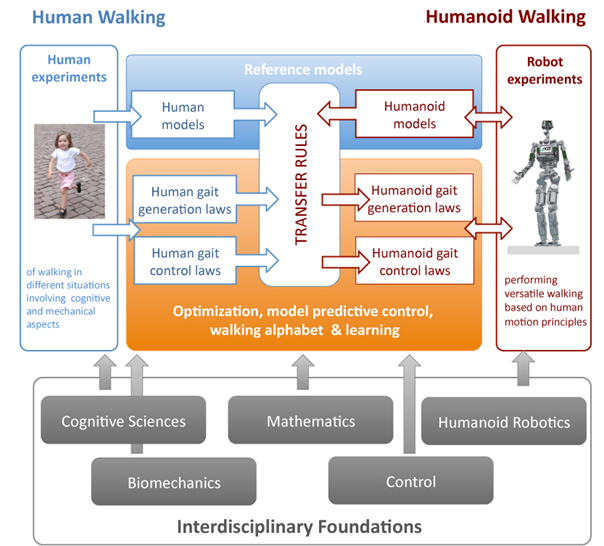
\includegraphics[width=0.8\linewidth]{figures/koroibot/components.png}
\caption{Graphical representation of the scientific approach of the \koroibot\ project.}
\label{fig:koroibot:components}
\end{figure}

\subsection*{Context}

This thesis has been written in the context of the European project \koroibot\ (\url{http://www.koroibot.eu/}).
The goal of the \koroibot\ project is to enhance the ability of humanoid robots to walk in a dynamic and versatile way, and to bring them closer to human capabilities.
As depicted in Fig.~\ref{fig:koroibot:components}, the \koroibot\ project partners have to study human motions and use this knowledge to control humanoid robots via optimal control methods.
Human motions are recorded with motion capture systems and stored in an open source data bank which can be found at \url{https://koroibot-motion-database.humanoids.kit.edu/}.
With these data several possibilities are exploited.
Assuming that humans minimize some criteria we can use inverse optimal control methods to find those criteria.
Walking alphabet and learning method \cite{Mandery2016b} are also used to transfer human behaviors to robots.
Finally, optimal control is used to build controllers that can eventually use these learned human behaviors while ensuring the robot safety.
Research and innovation works in \koroibot\ mainly target novel motion control methods for existing hardware.
It also derives optimized design principles for next robot generations.

\subsection*{\koroibot\ and robot challenges}

\begin{figure}
  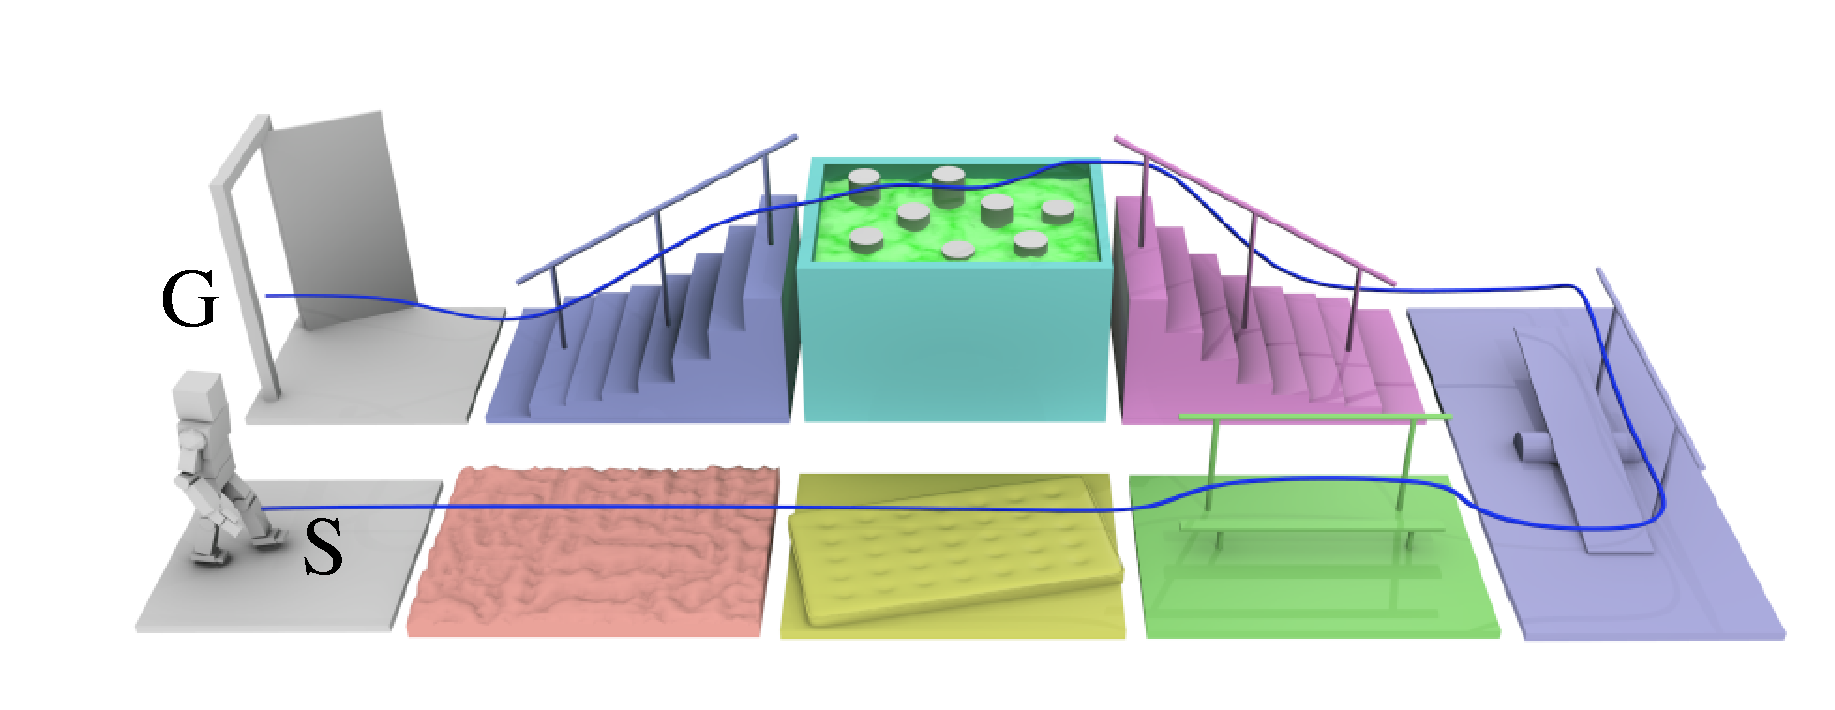
\includegraphics[width=\linewidth]{figures/KoroibotChallengeEnhanced.pdf}
  \begin{tikzpicture}[remember picture, overlay]
    %\draw[help lines] (0,0) grid (20,10);
    %\node at (0,0) {(0,0)};
    \draw[line width=1.5pt, color=red](2.5,2) ellipse (0.8cm and .6cm);
    \draw[line width=1.5pt, color=red](5.2,1.9) ellipse (1.1cm and .6cm);
    \draw[line width=1.5pt, color=red](11.5,1.9) ellipse (1.1cm and .6cm);
    \draw[line width=1.5pt, color=red](11,4) ellipse (1.1cm and .8cm);
    \draw[line width=1.5pt, color=red](5.6,4) ellipse (1.1cm and .8cm);
    \draw[line width=1.5pt, color=red](8.2,4.2) circle (1.0cm);
  \end{tikzpicture}
  \caption{Challenges of the \koroibot\ project. In red the challenges chosen by the LAAS-CNRS.}
  \label{fig:koroibot:scheme}
\end{figure}

In addition to this ambitious scientific aspect of the project, there is an important technical component.
Following the blue line in Fig.~\ref{fig:koroibot:scheme}, the different challenges of the project are to make humanoid robots:
\begin{list}{ \arabic{point}.}{%
		\usecounter{point}%
		\setlength{\topsep}{5pt}%
		\setlength{\itemsep}{0pt}%
		\setlength{\parsep}{0pt}%
		\setlength{\labelwidth}{3.em}%
		\setlength{\leftmargin}{2em}%
		\setlength{\labelsep}{0.5em}%
	}
\item[\bluesquare] walking on a flat ground,
\item[\bluesquare] walking on an uneven ground,
\item[\bluesquare] walking on a mattress,
\item[\bluesquare] walking on a beam with/without handrail,
\item[\bluesquare] walking on a seesaw with/without handrail,
\item[\bluesquare] climbing a stair case with/without handrail,
\item[\bluesquare] walking on stepping stones,
\item[\bluesquare] going down a stair case with/without handrail,
\item[\bluesquare] and walking through a door.
\end{list}
All the team owning a robot has to perform some of these challenges.
In Fig.~\ref{fig:koroibot:robots} we can see all the robot hosted by different partners.
Ideally, the algorithms developed in the frame of the \koroibot\ project has to be integrated on all the robots.
In practice the partners chose parts of the challenge to be realized on their different robotic platforms

\begin{figure}[ht]
\centering
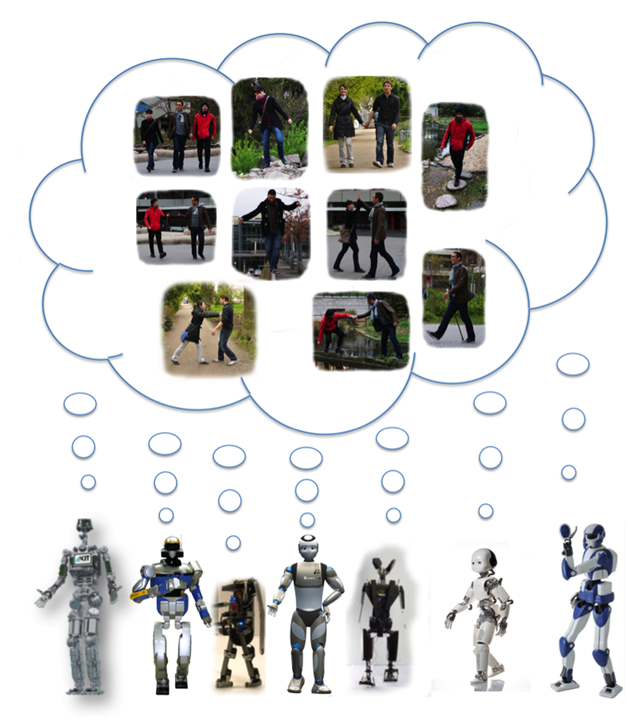
\includegraphics[width=0.7\linewidth]{figures/koroibot/situations_v2.png}
\caption{List of the humanoid robot used in the \koroibot\ project.}
\label{fig:koroibot:robots}
\end{figure}

\subsection*{\koroibot\ Key Performance Indicator (KPI)}

In the European project \koroibot\ we need to evaluate the improvement in terms of robot control and human likeness.
In this context and in collaboration with the H2R project, a detailed set of key performance indicators (KPI) have been proposed \cite{torricelli2015benchmarking}.
These KPI try to capture all the bipedal locomotion patterns.

A set of specific sub-function of the global motor behavior is analyzed (see Fig.~\ref{fig:koroibot:test}).
The different sub-function are divided in two.
First, the sub-function associated to body posture task with no locomotion.
And second the same sub-function but including the robot body transport.
The initial condition may vary depending on the experiment to perform.
This is the idea of the intertrial variability.
For example standing still on a horizontal flat surface is easy to reproduce at will.
Hence there is no intertrial variability.
On the contrary, while doing push recovery, it is difficult to reproduce the exact same push several times.
The sub-function are also classified taking into account the changes in the environment or not.

Each of these functions can be evaluated for different robots using the criteria depicted in Fig.~\ref{fig:koroibot:performance}.
The performance are classified in two sub categories, quantitative performance and human likeness.
In addition there are indications on the last two columns if the criteria is applicable on a standing task or on a locomotion task.

All the partners owning a humanoid robot need to perform an evaluation of these KPI.
However some movement are not possible yet on some robots of the consortium.
Hence, the different team picked meaningful criteria considering the current state of their robot and controllers.

\begin{figure}
\centering
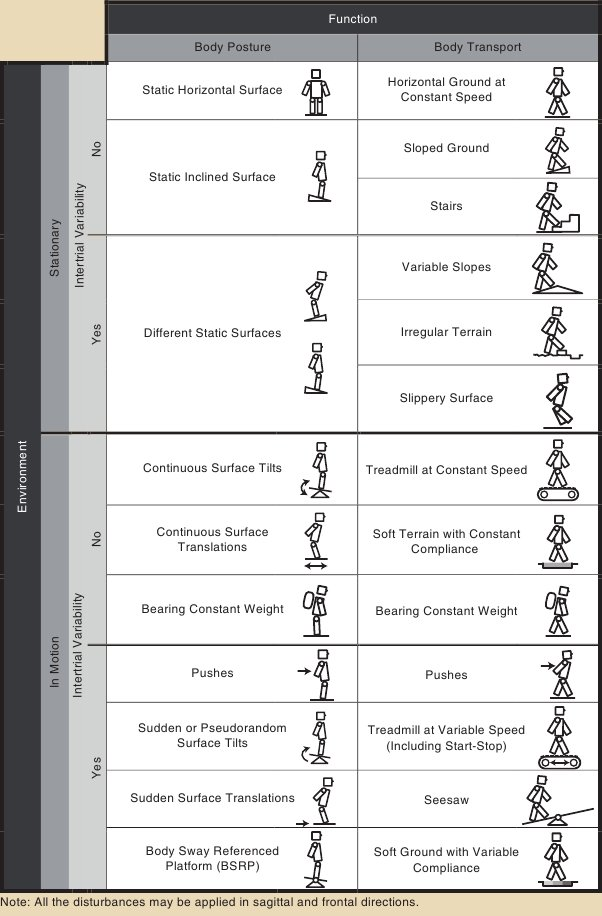
\includegraphics[width=0.9\linewidth]{figures/koroibot/KPIexperiment.jpg}
\begin{tikzpicture}[remember picture, overlay]
    %\draw[help lines, color=blue] (-8,0) grid (8,25);
    %\node [color=red] at (0,0) {\textbf (0,0)};
    %\node [color=red] at (0,20) {\textbf (0,20)};
    %\node [color=red] at (0,10) {\textbf (0,10)};
    \draw[line width=1.5pt, color=red](-3.9,19.7) ellipse (2cm and .5cm);
    \draw[line width=1.5pt, color=red](-3.9,16.9) ellipse (2cm and .5cm);
    \draw[line width=1.5pt, color=red](-3.9,9.0) ellipse (2cm and .5cm);
    \draw[line width=1.5pt, color=red](-9.5,7.25) ellipse (2cm and .5cm);
  \end{tikzpicture}
\caption{ The motor skills considered in the benchmarking scheme. This scheme is limited to bipedal locomotion skills. The concept of intertrial variability is
analogous to the concept of unexpected disturbances.
}
\label{fig:koroibot:test}
\end{figure}

\begin{figure}
\centering
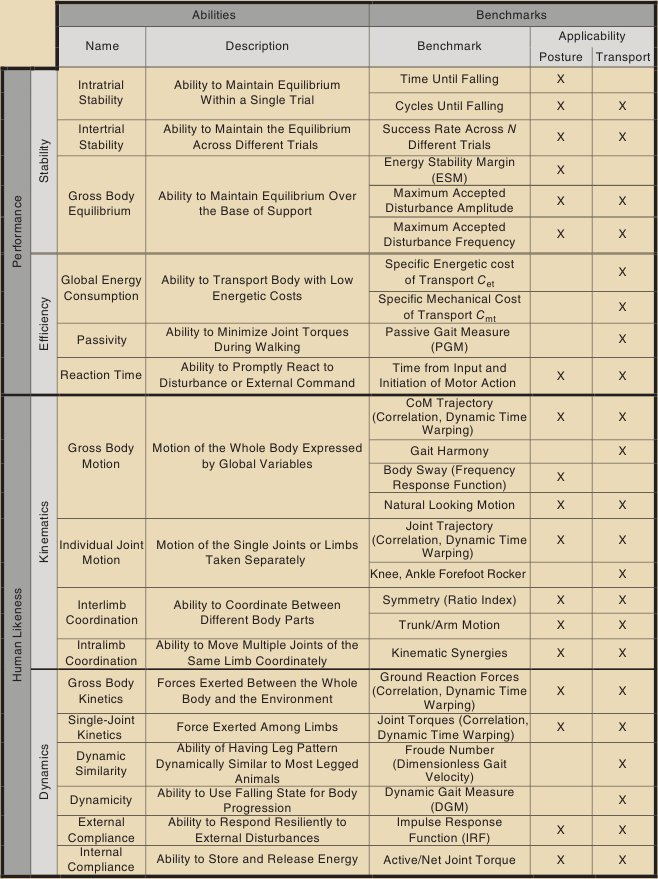
\includegraphics[width=0.90\linewidth]{figures/koroibot/KPIabilities.jpg}
\begin{tikzpicture}[remember picture, overlay]
    %\draw[help lines, color=blue] (-8,0) grid (8,25);
    %\node [color=red] at (0,0) {\textbf (0,0)};
    %\node [color=red] at (0,20) {\textbf (0,20)};
    %\node [color=red] at (0,10) {\textbf (0,10)};
    \draw[line width=1.5pt, color=red](-4.6,16.2) ellipse (2.2cm and .43cm);
    \draw[line width=1.5pt, color=red](-4.6,13.3) ellipse (2.2cm and .43cm);
    \draw[line width=1.5pt, color=red](-4.6,12.45) ellipse (2.2cm and .43cm);
  \end{tikzpicture}
\caption{The motor abilities and related benchmarks are classified in two categories: performance and human likeness. The
performance category includes all those abilities related to stability (ability of maintaining equilibrium) and efficiency. The human
likeness category includes all those abilities related to typical human behavior, under the perspective of kinematics and dynamics.
For each ability, a specific benchmark has been identified. The last column specifies in what classes of motor skills (i.e., the function
category of Fig.~\ref{fig:koroibot:test}) the corresponding benchmark is applicable.
}
\label{fig:koroibot:performance}
\end{figure}

\subsection*{The work done in the \koroibot\ context}

In LAAS-CNRS, the Gepetto team own the HRP-2 and the Romeo robots depicted respectively as the second and fourth robot in Fig.~\ref{fig:koroibot:robots} from the left to the right.
The Romeo robot is the first human size prototype of Softbank Robotics and has very limited locomotion capabilities.
Therefore I was in charge of integrating our algorithms on the HRP-2 robot.
Among the challenges from Fig.~\ref{fig:koroibot:scheme} we picked the one with a red circle, i.e:
\begin{list}{ \arabic{point}.}{%
		\usecounter{point}%
		\setlength{\topsep}{5pt}%
		\setlength{\itemsep}{0pt}%
		\setlength{\parsep}{0pt}%
		\setlength{\labelwidth}{3.em}%
		\setlength{\leftmargin}{2em}%
		\setlength{\labelsep}{0.5em}%
	}
\item[\bluesquare] walking on a flat ground,
\item[\bluesquare] walking on an uneven ground,
\item[\bluesquare] walking on a beam with/without handrail,
\item[\bluesquare] climbing a stair case with/without handrail,
\item[\bluesquare] walking on stepping stones,
\item[\bluesquare] and going down a stair case with/without handrail.
\end{list}
In addition to those challenges we added the perturbation rejection.
At the beginning of the project we evaluated the KPI on the HRP-2 robot.
In our case, we picked the KPI sub-functions meaningful considering the above selected challenges:
\begin{list}{ \arabic{point}.}{%
		\usecounter{point}%
		\setlength{\topsep}{5pt}%
		\setlength{\itemsep}{0pt}%
		\setlength{\parsep}{0pt}%
		\setlength{\labelwidth}{3.em}%
		\setlength{\leftmargin}{2em}%
		\setlength{\labelsep}{0.5em}%
	}
\item[\bluesquare] horizontal ground at constant speed,
\item[\bluesquare] stairs,
\item[\bluesquare] soft terrain with constant compliance,
\item[\bluesquare] bearing constant weight (the robot's own weight).
\end{list}
Coupled with the following benchmarks:
\begin{list}{ \arabic{point}.}{%
		\usecounter{point}%
		\setlength{\topsep}{5pt}%
		\setlength{\itemsep}{0pt}%
		\setlength{\parsep}{0pt}%
		\setlength{\labelwidth}{3.em}%
		\setlength{\leftmargin}{2em}%
		\setlength{\labelsep}{0.5em}%
	}
\item[\bluesquare] success rate across N different trials,
\item[\bluesquare] specific energy cost of transport,
\item[\bluesquare] specific mechanical cost of transport,
\end{list}
All these choices are shown in the tables from Fig.~\ref{fig:koroibot:test} and Fig.~\ref{fig:koroibot:performance} by red ellipses.
The mathematical details and results are presented below in section {"\koroibot\ Key Performance Indicator (KPI)"}.

\paragraph*{Reactive walking}
The results pointed out some interesting points.
First the ground walking velocity and versatility of HRP-2 can be improved.
In this context we did a collaboration, presented in Chap.~\ref{chap:nmpc}, with our mathematician colleagues from the University of Heidelberg.
This collaboration leads to a new real time walking pattern generator with increased functionalities like obstacle avoidance.
In addition to this, the implementation of the dynamic filter, presented by Nishiwaki and al. in \cite{Nishiwaki:IJRR:09}, increase the range of the reachable CoM velocity.
\paragraph*{Multicontact motion generation}
The second problem that arose from the KPI was the energy consumption during the stair climbing.
One possible way for solving this problem is to distribute the robot weight over multiple contacts.
Hence, we designed an innovative multi-contact controller to allow generic locomotion and the use of a handrail.
Chap.~\ref{chap:multicontact} explains this contribution in details.
\paragraph*{Fire hose manipulation}
The second application concerns perturbation rejection and has been done in a collaboration with the Japanese national institute of Advanced Industrial Science and Technology (AIST).
This application is inspired from the DARPA robotic challenge.
The idea of this work is to see if a humanoid robot with average power and size like HRP-2 is able, using a state of the art controller, to pull a stiff fire hose.
The details of the experiment are written in Chap.~\ref{chap:hose}
\paragraph*{One third power law}
In the frame of the \koroibot\ project, researchers studied the human motion to extract quantitative data.
In fact they noticed that humans adapt their velocities in function of the curvature of their trajectories.
The scientific question that we tried to answer is the following: "Can this law extracted from human motion help humanoid robots to walk ?" 
A fruitful collaboration with these experts allowed us to answer this question.
This resulted in the design of an innovating controller for tracking cyclic trajectories of the center of mass.
Chap.~\ref{chap:powerlaw} present this work in details.
\paragraph*{Human motion primitives and model predictive control}
Another collaboration with human motion experts was done to study if motion primitives extracted from human behavior could be applied to humanoid robot.
To answer this question we propose a whole body controller using upper body movement primitives extracted from human behavior and lower body movement computed by a walking pattern generator.
Chap.~\ref{chap:primitives} show these fused bottom up and top down approaches.
\paragraph*{Reactive controllers}
In this thesis we studied reactive behavior for humanoid robot.
We designed applications that make the robot facing real case scenarios.
The first application was done in the frame of a collaboration with Airbus/Future of Aircraft Factory.
The idea was to build controllers for test case scenarios and evaluate if humanoid robot could go in a factory.
We used online planner for obstacle avoidance, visual servoing coupled with a walking pattern generator to place the robot in a desired position, a whole body controller for screwing tasks, and center of pressure based walking pattern generator to climb stairs.
Chap.~\ref{chap:univworker} explains this contribution in details.
